\section{Specific Requirements}
	\subsection{External Interface Requirements}
		\subsubsection{API Interfaces}
			For taxi waiting time and other minor features we decided to use Google Maps API.
			It is a very powerful library that perfectly fits our needs.
			When a taxi accepts a request, the system retrieves its position and, through
			those APIs, is able to process either the hypothetical route that the taxi will
			follow to reach the passenger's position and, consequently, the arrival time.
			The system will, then, forward those information to the passenger.
		\subsubsection{Hardware Interfaces}
			Our project includes a web and a mobile application, so it does not require
			any external hardware interface.
		\subsubsection{Software Interfaces}
			\begin{itemize}
				\item Database Management System (DBMS):
				\begin{itemize}
					\item Name: MySQL.
					\item Version: 5.6.21
					\item Source: http://www.mysql.it/
				\end{itemize}
				\item Java Virtual Machine (JVM).
				\begin{itemize}
					\item Name: JEE
					\item Version: 7
					\item Source: http://www.oracle.com/technetwork/java/javaee/tech/index.html
				\end{itemize}
				\item Application server:
				\begin{itemize}
					\item Name: Glassfish.
					\item Version: 4.1.
					\item Source: https://glassfish.java.net/
				\end{itemize}
				\item Operating System (OS).
				\begin{itemize}
					\item Application must be able to run on any SO which supports JVM and DBMS specified before.
				\end{itemize}
			\end{itemize}
		\subsubsection{Communication Interfaces}
			\begin{center}
				\begin{tabular}{ | l | l | l | p{5cm} |}
					\hline
					Protocol & Application & Port 	\\ \hline
					TCP & HTTPS & 443				\\ \hline
					TCP & HTTP  & 80				\\ \hline
					TCP & DBMS  & 3306 (default)	\\ \hline
				\end{tabular}
			\end{center}
	\subsection{Functional Requirements}
		\subsubsection{Permit a guest to register to the service}
			\begin{enumerate}[label=\bfseries R\arabic*:]
				\item Guest can access registration form.
				\item Guest must not be already registered to perform registration process.
				\item Guest must choose a unique username (never used by other users)
				\item Guest can not sign up twice but only once for session.
				\item During registration must provide all necessary information
			\end{enumerate}
		\subsubsection{Permit a guest to request a taxi}
			\begin{enumerate}[label=\bfseries R\arabic*:]
				\item Guest must provide basic personal information
				\item Guest must agree to provide his position
			\end{enumerate}
		\subsubsection{Permit a guest to sign in}
			\begin{enumerate}[label=\bfseries R\arabic*:]
				\item User must be already registered to sign in.
				\item User must provide login information to complete the operation.
				\item The couple username and password inserted during login process must be correct
					(the same couple inserted during registration).
				\item Wrong credentials will not grant the access.
				\item After the login operation, the user will be treated as a registered passenger.
				\item After the login operation, the registration form will not be available for the current session.
			\end{enumerate}
		\subsubsection{Permit a registered passenger to require a taxi}
			\begin{enumerate}[label=\bfseries R\arabic*:]
				\item User must be already registered and logged in the application.
				\item User must agree to provide his position.
				\item No additional information is required.
			\end{enumerate}
		\subsubsection{Permit a registered passenger to make a reservation}
			\begin{enumerate}[label=\bfseries R\arabic*:]
				\item User must be already registered and logged in the application.
				\item User must make a reservation at least 2 hours before the request time.
				\item User must provide time, origin and destination of the ride at the moment of the reservation.
				\item User must confirm the reservation process.
				\item The reservation can be deleted by the user himself.
			\end{enumerate}
		\subsubsection{Permit a registered passenger to cancel a reservation}
			\begin{enumerate}[label=\bfseries R\arabic*:]
				\item User must be already registered and logged in the application.
				\item User can delete only a reservation made by himself.
				\item User can not delete a reservation within 10 minutes before the time of the request.
				\item User must confirm the deleting process.
				\item Deleting process is not reversible.
			\end{enumerate}
		\subsubsection{Permit a taxi driver to give the system his availability}
			\begin{enumerate}[label=\bfseries R\arabic*:]
				\item User must use the mobile application.
				\item User must be already registered and logged in the application.
				\item User must be a taxi driver.
				\item The taxi driver must be unavailable.
			\end{enumerate}
		\subsubsection{Permit a taxi driver to revoke his availability}
			\begin{enumerate}[label=\bfseries R\arabic*:]
				\item User must use the mobile application.
				\item User must be already registered and logged in the application.
				\item User must be a taxi driver.
				\item The taxi driver must be available.
			\end{enumerate}
		\subsubsection{Permit a taxi driver to accept or refuse a ride request}
			\begin{enumerate}[label=\bfseries R\arabic*:]
				\item User must use the mobile application.
				\item User must be already registered and logged in the application.
				\item User must be a taxi driver.
				\item The taxi driver must be available.
				\item the taxi driver must have received a notification for that ride request.
			\end{enumerate}
	\subsection{Scenarios}
		\subsubsection{Occasional user}
			Mario, an important businessman, has just arrived by train in our city for the first time.
			His train had technical issues and now he is a bit late for the meeting on 
			the opposite side of our town, so he does not want to take public transports.
			The best solution is to call a taxi.
			He opens the browser on his smartphone and, inserting name and surname, sends a taxi request
			to our system. As soon as possible he receives a notification with the taxi ID number and the
			waiting time before the taxi arrival. In less than no time he will reach the meeting location.
		\subsubsection{Habitual user}
			The meeting of Mario went very well: he started an important collaboration with a local
			company. He will have to come back often in our town. He found our service very useful, so
			he decides to register and download the mobile application. After a couple of weeks he has to
			come back. Unfortunately his train had technical issues, and he risks to be late to the
			meeting again. This time he has our application installed on his mobile device, so with only
			few taps and no additional information provided requires a taxi. As soon as possible he receives
			a notification with the taxi ID number and the	waiting time before the taxi arrival.
			In less than no time he will reach the meeting location.
		\subsubsection{Taxi reservation}
			After another couple of weeks, Mario has to come back in our town again. He thinks that he 
			will never be so unlucky to find a defective train for the third consecutive time,
			so he decides to make a reservation before leaving,	in order to find a taxi waiting for him
			at the train station at his arrival. Using the mobile application, he fills in all the
			necessary fields, indicating hour and place of the request.
			Now he can airily taste	his journey.
		\subsubsection{Deleting a taxi reservation}
			Mario's train has technical issues. Poor Mario, he's so unlucky! He will be very late, 
			so he does not want to let the taxi wait so long. He opens our application and, 30 minutes
			before the taxi request, he selects the reservation and deletes it. Once arrived he will
			require a taxi as usual.
		\subsubsection{Taxi driver}
			A taxi driver, Luigi, is having a little break, eating his favourite chocolate bar in his taxi. Suddenly
			his phone rings: a notification has just arrived. But he's having a break, so he does not answer.
			After 1 minute, the system automatically records a negative answer from the taxi driver.
			Luigi slowly ends his bar and starts answering some messages on his smartphone. Suddenly his phone
			rings. He sees the notification, but he's very busy, so he declines the request. Luigi greets his
			friend on the chat and goes back to work. After a few minutes his phone rings again. A man called
			Mario is requesting a taxi in his area, right next to the train station. He accepts the request and
			starts driving towards the location of the customer.
		\subsubsection{Taxi availability}
			After a hard morning, Luigi decides that it is the right time to have lunch. He opens our mobile
			application and sets his status as unavailable: he does not want to be disturbed during such an
			important moment. After a hearty lunch, he goes back to work, so he picks up his phone, opens our
			application and sets his status as available. He works hard for the whole afternoon and, after the
			last passenger, he's so tired that he forgets the status on available. The system sends him 1, 2, 3
			notifications of requests, but Luigi has a huge headache and can not hear the phone ringing. After
			the third request without answer the system automatically sets the driver as unavailable.
			Finally Luigi will get its deserved peace.
	\newpage
	\subsection{Use Case Diagram}
		\begin{figure}[h!]
			\centering
			\graphicspath{ {../SE2_IMAGES/} }
			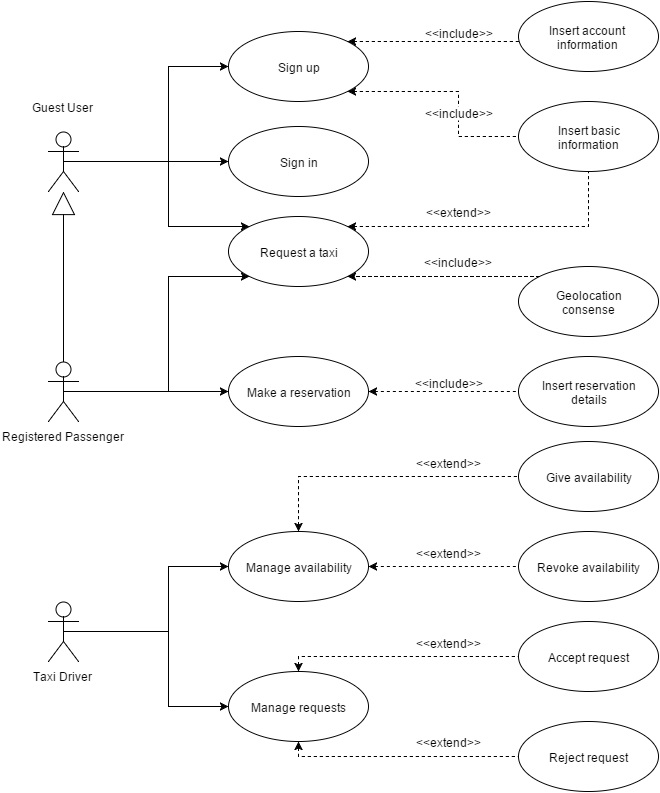
\includegraphics[width=\linewidth]{UseCase.jpg}
			\caption{Use Case Diagram for MyTaxiService}
		\end{figure}
	\newpage
	\subsection{Class Diagram}
		\begin{figure}[h!]
			\centering
			\graphicspath{ {../SE2_IMAGES/} }
			\includegraphics[width=\linewidth]{ClassDiagram.png}
			\caption{Class Diagram for MyTaxiService}
		\end{figure}